\documentclass{article}

% if you need to pass options to natbib, use, e.g.:
%     \PassOptionsToPackage{numbers, compress}{natbib}
% before loading neurips_2024


% ready for submission
\usepackage[preprint]{neurips_2024}


% to compile a preprint version, e.g., for submission to arXiv, add add the
% [preprint] option:
%     \usepackage[preprint]{neurips_2024}


% to compile a camera-ready version, add the [final] option, e.g.:
%     \usepackage[final]{neurips_2024}


% to avoid loading the natbib package, add option nonatbib:
%    \usepackage[nonatbib]{neurips_2024}


\usepackage[utf8]{inputenc} % allow utf-8 input
\usepackage[T1]{fontenc}    % use 8-bit T1 fonts
\usepackage{hyperref}       % hyperlinks
\usepackage{url}            % simple URL typesetting
\usepackage{booktabs}       % professional-quality tables
\usepackage{amsfonts}       % blackboard math symbols
\usepackage{nicefrac}       % compact symbols for 1/2, etc.
\usepackage{microtype}      % microtypography
\usepackage{xcolor}         % colors
\usepackage{graphicx}


\title{What is the best Augmentation for Generalization?}


% The \author macro works with any number of authors. There are two commands
% used to separate the names and addresses of multiple authors: \And and \AND.
%
% Using \And between authors leaves it to LaTeX to determine where to break the
% lines. Using \AND forces a line break at that point. So, if LaTeX puts 3 of 4
% authors names on the first line, and the last on the second line, try using
% \AND instead of \And before the third author name.


\author{%
  SungWoo Cho \\
  \texttt{paion0603@gmail.com} \\
}


\begin{document}


\maketitle


\begin{abstract}
    There comes a point in everyone's life when they wonder what the best augmentation technique is. Is there an obvious answer or there something I'm not aware of? This study was an abliation study using a total of five methods to address this question. The five methods are 1. No Augmentation 2. basic Augmentation 3. basic Augmentation + Mixup 4. basic Augmentation + CutMix 5. All Random, and the dataset is Stanford Dogs and the model is ResNet-50.
\end{abstract}


\section{Introduction}


Data Augmentation in Computer Vision improves generalization performance. Data augmentation artificially increases the diversity of the training dataset to help the model learn more diverse input patterns. This, in turn, improves the model's ability to generalize to data it hasn't seen. It's an effective way to prevent overfitting, especially in data-limited environments[1,2,3]. However, there is a lack of specific guidelines on which augmentations are best. This paper aims to provide the foundation for a paper that will reveal which augmentations are effective in different situations.     

    \begin{figure}[h]
      \centering
      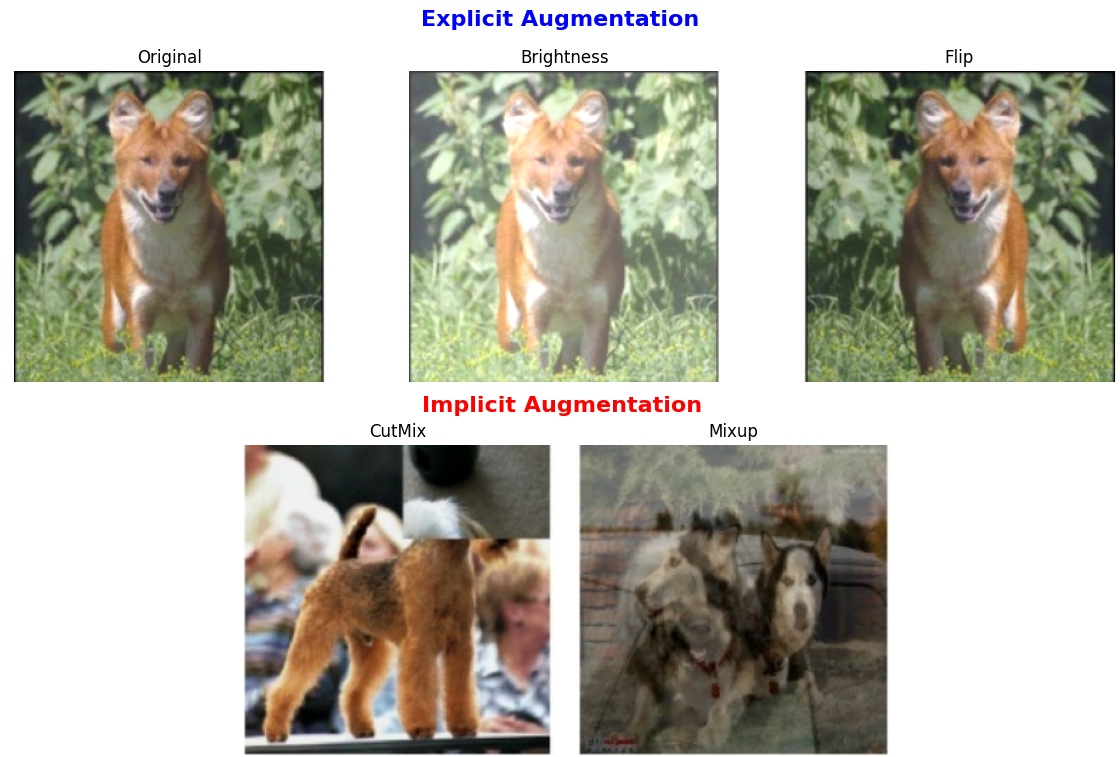
\includegraphics[width=\linewidth]{Augmentation.jpg}
      \caption{Example of Explicit \& Implicit Augmentation}
    \end{figure}
    

\subsection{Explicit Augmentation}


Explicit augmentation is a technique for increasing the diversity of a dataset by explicitly transforming the data. This is often done by {\bf cropping, flipping, coloring}, etc. and is useful to improve the generalization performance of a model and prevent overfitting [1]. Explicit augmentation techniques, such as cropping, flipping, and coloring, are effective in improving a model’s generalization by artificially increasing the diversity of the dataset. However, these methods have inherent limitations. For instance, they are constrained by the transformations applied to the original data—meaning they cannot create fundamentally new variations beyond what the explicit rules allow. Consider an image classification task: if all images of a cat in the dataset are photographed from a similar angle, explicit augmentation methods like rotation or mirroring can only provide limited diversity. They cannot generate an image of the same cat from an entirely new viewpoint.


\subsection{Implicit Augmentation}

To overcome these constraints, implicit augmentation techniques have been developed. The key difference between Explicit Augmentation and Implicit Augmentation is {\bf Label-Preserving} and {\bf Label-Transforming}. Explicit augmentation preserves the labels of the original image so that the trained model can still classify the transformed image correctly. Implicit augmentation, however, adds transformations to the labels to create a new data distribution, which encourages the model to learn more general patterns. The two different variations can be seen in Figure 1.


\section{Methods}
\label{gen_inst}


We used a total of five methods to compare which augmentations yield the best generalization performance. The first is no-Augmentation. We used the performance of the model without augmentation as a baseline to see if augmentation improves performance. The second is basic-Augmentation. This method utilizes only explicit augmentation and applies random horizontal flip and random brightness adjustment. The third method applied CutMix to basic-Augmentation, and the fourth method applied Mixup to basic-Augmentation. Finally, the fifth method randomizes all of the augmentations.

We used the Stanford Dogs dataset, which consists of 120 different dog breeds labeled accordingly. The dataset contains a total of 20,580 images, with 12,000 images used for training and 8,580 images for testing. To create a validation set, we split the training set into 80\% training data and 20\% validation data.

For the model, we used ResNet-50, leveraging pre-trained weights from ImageNet. Each case's optimal model checkpoint was determined based on validation accuracy. In this approach, only the Classifier layers participated in the training process, while the pre-trained backbone network parameters remained frozen.


\section{Result}
\label{headings}

Table \ref{model-performance} presents the test and validation accuracy of five augmentation strategies.

First, {\bf explicit augmentation} (random flipping and brightness adjustment) showed the highest test accuracy (74.50\%), outperforming the baseline (No Augmentation) by 1.2\%. This confirms that explicit augmentation improves model generalization by introducing more diverse training samples.

However, {\bf implicit augmentation} techniques such as Mixup and CutMix resulted in lower performance. The Augmentation + Mixup method yielded the lowest test accuracy (64.74\%), while Augmentation + CutMix also performed worse than explicit augmentation alone (69.09\%).  This suggests that label mixing techniques(Label-Transforming) are not suitable for the Stanford Dog dataset. The Stanford Dog dataset also suggests that it is likely important to retain spatial and structural information to distinguish between classes, and that label mixture techniques may not be suitable for fine-grained classification tasks.

Additionally, the Random Augmentation strategy (which applied a mix of transformations without a structured approach) did not perform well, achieving a test accuracy of 65.35\%. This indicates that applying augmentations arbitrarily may not always lead to improved generalization. Instead, carefully selecting augmentation techniques based on dataset characteristics is essential for maximizing model performance.

These findings demonstrate that while data augmentation is generally beneficial, its effectiveness depends on the specific technique used. Explicit augmentation methods remain a reliable choice, whereas implicit augmentation techniques should be applied selectively based on the dataset and task requirements.



\begin{table}[h]
  \caption{Comparison of Model Performance}
  \label{model-performance}
  \centering
  \begin{tabular}{lcc}
    \toprule
    Method              & Test Accuracy (\%) & Validation Accuracy(\%) \\
    \midrule
    Augmentation        & 74.50         & 73.42            \\
    No Augmentation     & 73.30         & 71.58            \\
    Aug + CutMix        & 69.09         & 67.79            \\
    Random              & 65.35         & 63.88            \\
    Aug + MixUp         & 64.74         & 66.75            \\
    \bottomrule
  \end{tabular}
\end{table}


\section{Conclusion}
\label{others}


This study investigated the effectiveness of different augmentation techniques in improving model generalization. The results demonstrate that explicit augmentation methods, such as random flipping and brightness adjustment, consistently enhance model performance. However, implicit augmentation techniques, such as Mixup and CutMix, did not yield improvements and, in some cases, even degraded performance. This suggests that label-mixing techniques may not be well-suited for fine-grained classification tasks where preserving spatial structure is crucial.

Furthermore, the findings highlight the importance of selecting augmentation strategies based on the {\bf dataset characteristics} rather than applying augmentations arbitrarily. While augmentation remains a powerful tool for improving generalization, not all techniques are universally beneficial across different tasks.

However, this study has a key limitation: it does not provide a definitive answer as to which augmentation method is the best in all scenarios. Instead, it emphasizes that the optimal augmentation technique depends on the dataset. If we could predict the most suitable augmentation strategy for a given dataset in advance, it would represent a significant breakthrough in the field of data augmentation. We hope that future research will explore this direction, developing methodologies to systematically determine the best augmentation strategies for different datasets.


\section*{References}


\medskip

[1] Krizhevsky, A., Sutskever, I., \& Hinton, G.E. (2012) ImageNet Classification with Deep Convolutional Neural Networks. In F. Pereira, C.J.C. Burges, L. Bottou, \& K.Q. Weinberger (eds.), {\it Advances in Neural Information Processing Systems 25}. Curran Associates, Inc.


[2] Zhang, H., Cissé, M., Dauphin, Y.N., \& Lopez-Paz, D. (2017) mixup: Beyond Empirical Risk Minimization. arXiv preprint arXiv:1710.09412.

[3] Yun, S., Han, D., Oh, S.J., Chun, S., Choe, J., \& Yoo, Y. (2019) CutMix: Regularization Strategy to Train Strong Classifiers With Localizable Features. In {\it Proceedings of the IEEE/CVF International Conference on Computer Vision (ICCV)}, October 2019.

\end{document}